\subsection{The basic sorting algorithm}\par

The actual sorting functionality is mostly done by two basic algorithms, similar and diverse shuffle.\par

 \begin{figure}[H] 
	\centering
	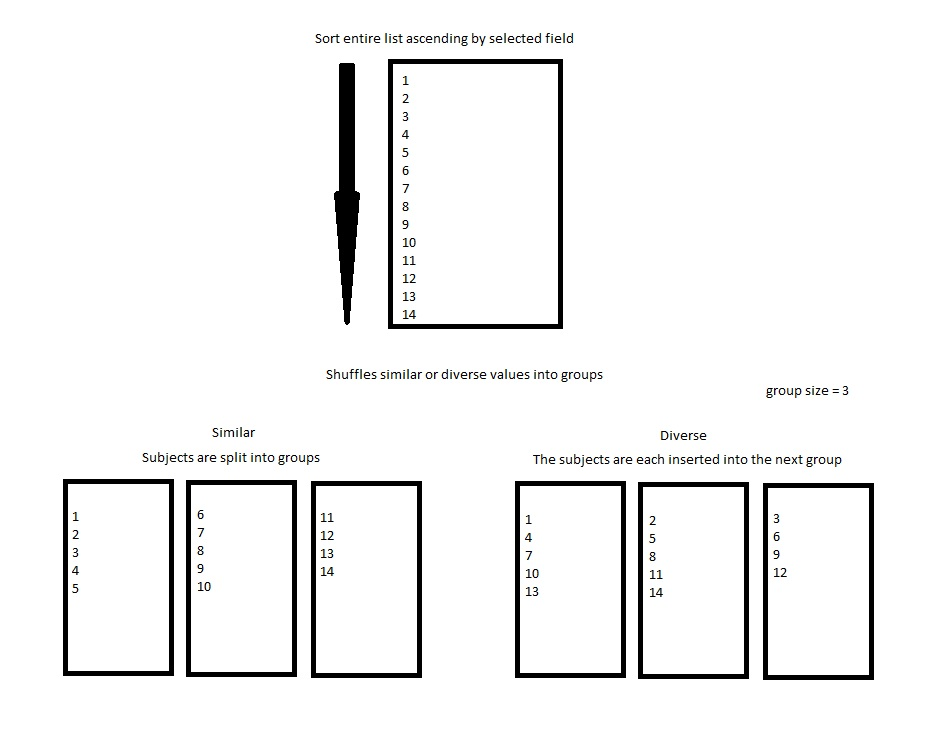
\includegraphics[width=12cm]{./graphics/basicAlgorithm.jpg}\par
	\caption{The basic similar/diverse shuffle algorithm}
\end{figure}
With both functions the list of subjects are sorted in ascending order, by the selected field.

The similar algorithm then splits the list of subjects into a predefined number of groups as blocks, and the diverse algorithm inserts each of the subjects into the next group in the linked list. 



\subsection{Shuffling by a single field}\par

Selecting a single field runs the basic algorithm only once.\par
 \begin{figure}[H] 
	\centering
	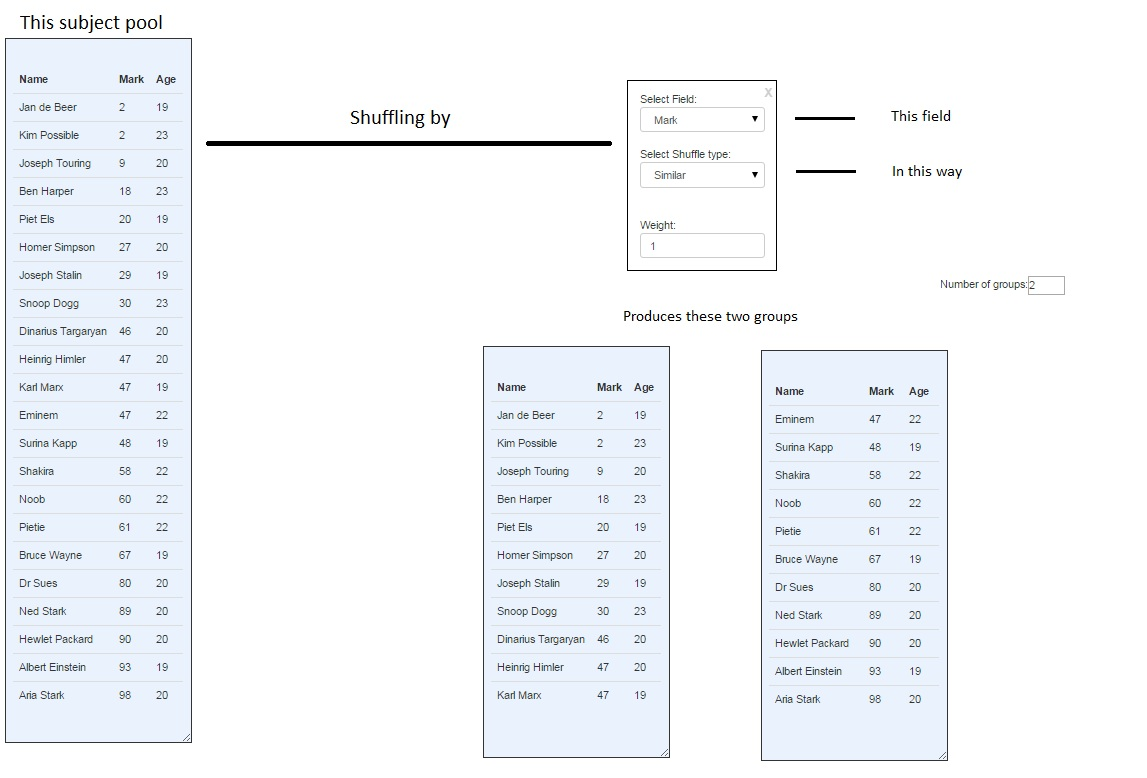
\includegraphics[width=16cm]{./graphics/singleField.jpg}\par
	\caption{Single field example}
\end{figure}

With only one field selected as criteria, weight is irrelevant. Distribution is as good as it's going to get for the selected field.

\subsection{Shuffling by multiple fields}\par

Multi-level shuffling is used, the field with the highest weight(or first in line),
is used to pre-shuffle the subjects into a smaller amount of teams,which are then each sorted into teams to finally reach the desired amount of teams.
  \par
 \begin{figure}[H] 
	\centering
	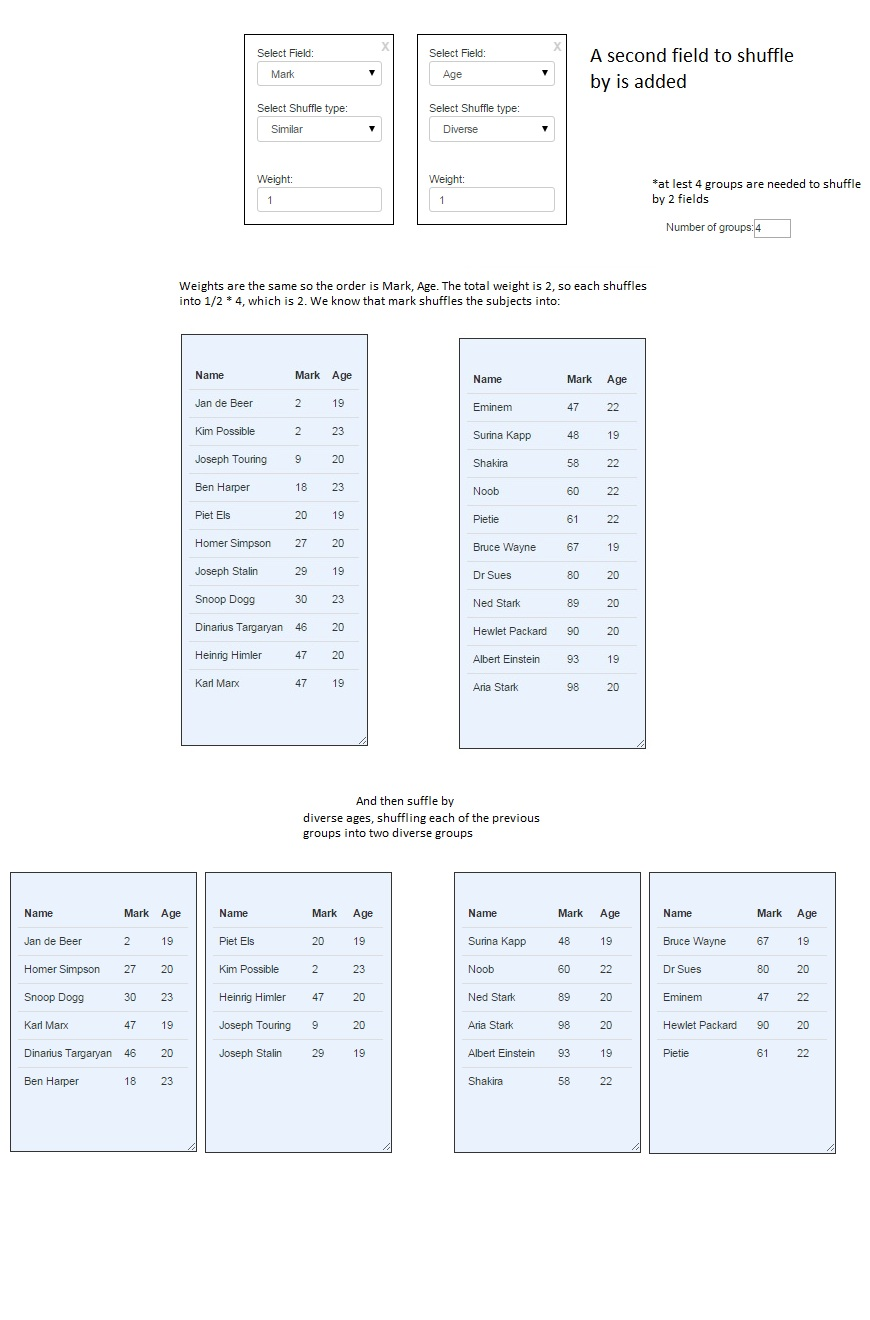
\includegraphics[width=16cm]{./graphics/multipleField.jpg}\par
	\caption{Multiple field example}
\end{figure}